\section{Sigma-Delta-Wandler}

\begin{minipage}{0.45\linewidth}
    \begin{tabular}{ll}
        $n$ & Anzahl Bits \\
        $D$ & Digitaler Wert \quad $D < 2^n$ \\
        $q$ & Quantisierungsschritt \\
        $B_0$ & Bitwert 0 (LSB) \\
        $B_{n-1}$ & Bitwert $n-1$ (MSB)
    \end{tabular}
\end{minipage}
\hfill
\begin{minipage}{0.42\linewidth}
    $ \boxed{ q = \frac{V_{\rm refp} - V_{\rm refn}}{2^n} } $ \\
    $ \boxed{ D = \frac{V_{\rm in} - V_{\rm vrefn}}{V_{\rm refp} - V_{\rm refn}} \, 2^n }  $
\end{minipage}


\subsection{Single-Slope-Wandler}

% TODO


\subsection{Dual-Slope-Wandler}

% TODO: formatting / adjustments

\begin{minipage}{0.42\linewidth}
    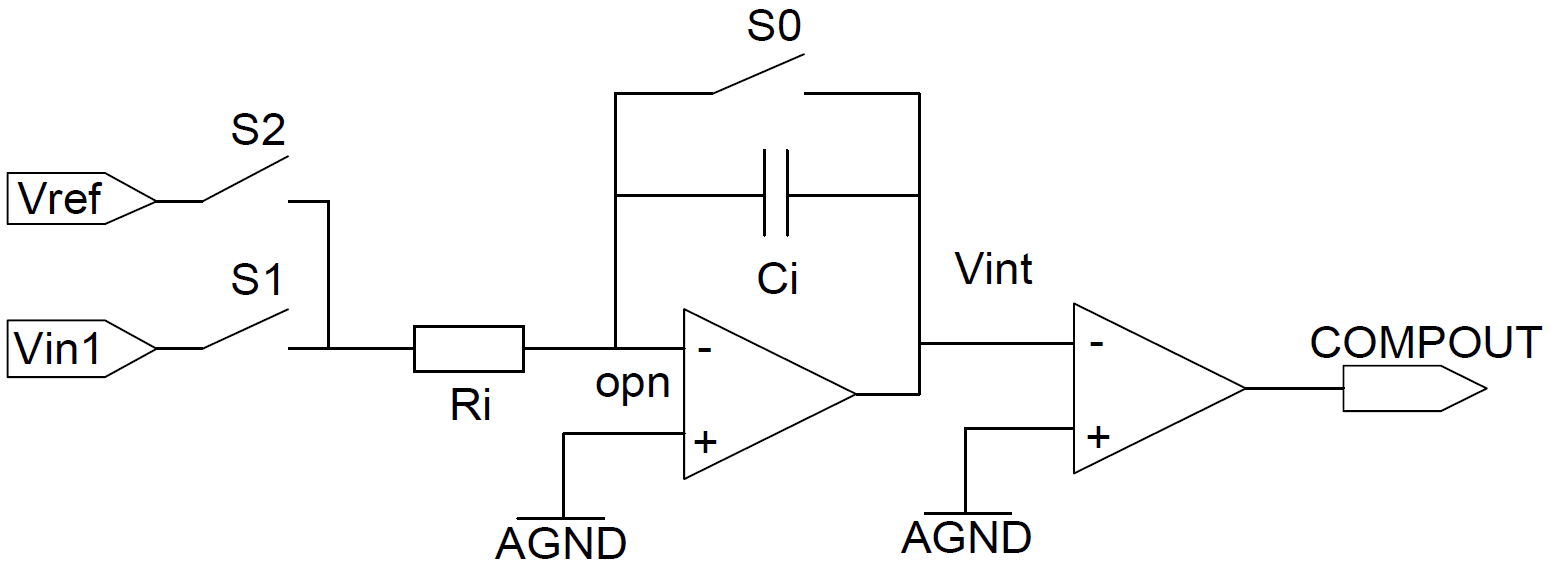
\includegraphics[width=\linewidth]{images/dual_slope_ADC}
\end{minipage}
\hfill
\begin{minipage}{0.27\linewidth}
    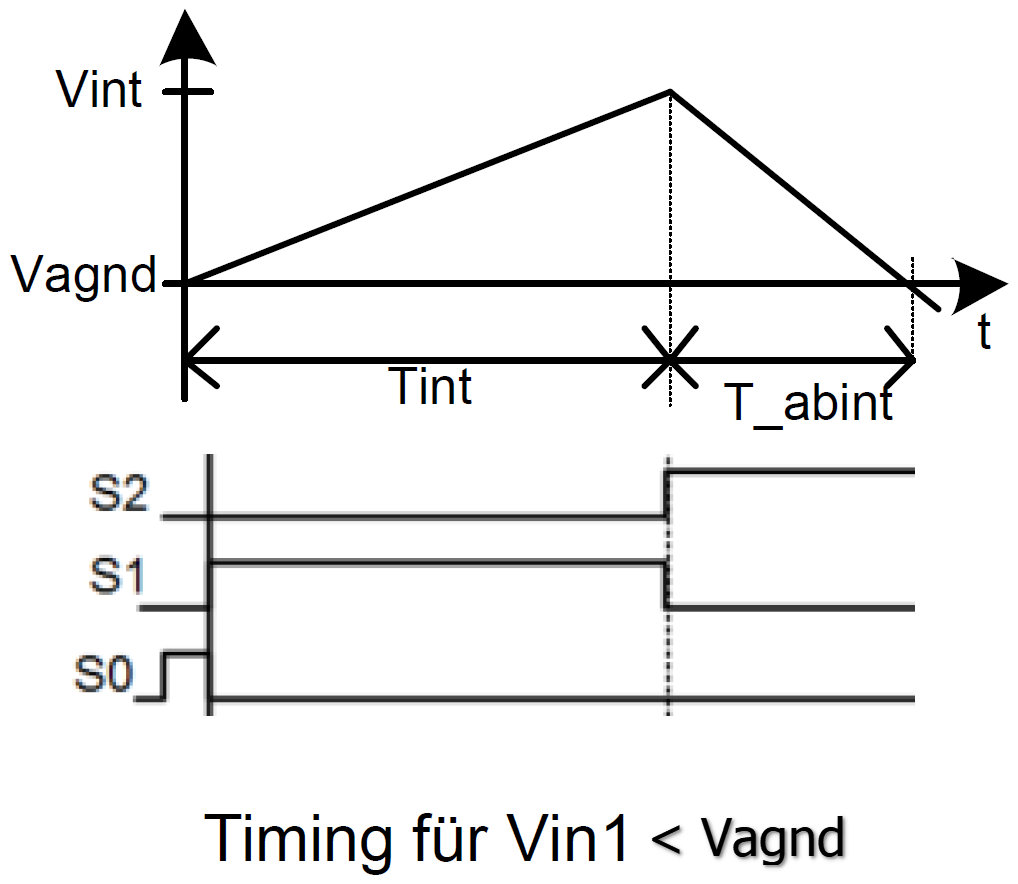
\includegraphics[width=0.83\linewidth]{images//dual_slope_ADC_timing}
\end{minipage}
    \hfill
\begin{minipage}{0.29\linewidth}
    $ \boxed{  V_{\rm int} = \frac{\overline{V_{\rm in}} \cdot T_{\rm int}}{R_i \cdot C_i} } $ 
    $ \boxed{  V_{\rm abint} = \frac{V_{\rm ref} \cdot T_{\rm abint}}{R_i \cdot C_i}  } $ 
\end{minipage}
    
$ \boxed{ \text{DC: } V_{\rm int} = V_{\rm AGND}- \frac{1}{R_i \cdot C_i} \, (V_{\rm in1}- V_{\rm AGND}) \cdot T_{\rm int} } $ 
\quad $\boxed{ \Delta V_{\rm abint} = - \Delta V_{\rm int} }$ \\
$ \boxed{ \Delta V_{\rm abint} = V_{\rm AGND} - V_{\rm int} = - \frac{1}{R_i \cdot C_i} \, (V_{\rm ref} - V_{\rm AGND}) \cdot T_{\rm abint} }$ 
\quad $\boxed{ T_{\rm abint} = - \frac{V_{\rm in1} \cdot T_{\rm int}}{V_{\rm ref}} }$\\
  
$\boxed{\text{Allgemein: } V_{\rm int} = \int\limits_0^{T_{\rm int}} - \frac{1}{R_i \cdot C_i} \, V_{\rm in1} + V_{\rm int,0} }$
\quad 
$ \boxed{ -\frac{\overline{V_{\rm in}}}{V_{\rm ref}}= \frac{T_{\rm abint}}{T_{\rm int}} = \frac{n \cdot T_{\rm clk}}{N \cdot T_{\rm  clk} } }$




\subsubsection{Frequenzverhalten vom Dual-Slope-Wandler}

Frequenzen $f = \frac{1}{T}$ , wobei $T$ der Intergrationszeit entspricht, werden perfekt unterdrückt \\
$\Rightarrow$ Integrationszeit $T = 20 \, \mathrm{ms}$ unterdrückt Netzbrumm von $50 \, \mathrm{Hz}$


\subsection{Sigma-Delta-Wandler}


\begin{minipage}[c]{0.48\columnwidth}
    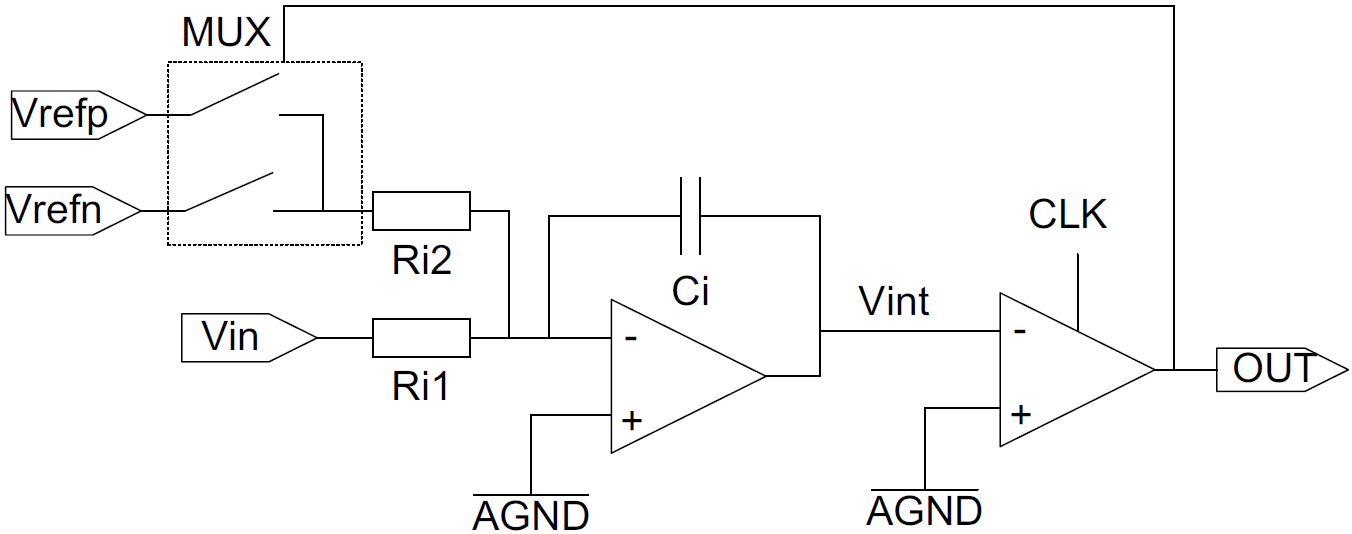
\includegraphics[width=\columnwidth]{images/sigma-delta-wandler.png}
\end{minipage}
\hfill
\begin{minipage}[c]{0.48\columnwidth}
    $$ \boxed{V_{\rm in} = \frac{2 \cdot n  - N}{N} V_{\rm ref}} $$

    \begin{tabular}{ll}
        $N$ & \# Taktzyklen von Clk \\
        $n$ & \# Taktzyklen, in denen \\
            & Modulator-Ausgang $=1$
    \end{tabular}
\end{minipage}
